\documentclass[12pt,twoside,space]{ctexart}
\usepackage{NEMT}
\usepackage{float}
\begin{document}\zihao{5}
\juemi
\biaoti{试卷1}
\fubiaoti{副标题1}
{\heiti 注意事项}
\begin{enumerate}[itemsep=-0.3em,topsep=0pt]
\item 答卷前,考生务必将自己的姓名和准考证号填写在答题卡上。
\item 回答选择题时,选出每小题答案后,用铅笔把答题卡对应题目的答案标号涂黑。如需改动,用橡皮擦干净后,再选涂其它答案标号。回答非选择题时,将答案写在答题卡上。写在本试卷上无效。
\item 考试结束后,将本试卷和答题卡一并交回。
	请认真核对监考员在答题卡上所粘贴的条形码上的姓名、准考证号与您本人是否相符。
\end{enumerate}
\section{解答题:本题共1个小题,共10分}
\begin{enumerate}[itemsep=0.2em,topsep=0pt]
\item
如图,抛物线$ y=\frac{1}{5}x^2-\frac{16}{5} $与x轴交与A,B两点,顶点为C,点P在抛物线上,且位于x轴下方。已知P(1,-3),B(4,0),若点D是抛物线上的一点,满足$ \angle DPO=\angle POB $,求点D的坐标。
\begin{figure}[H]
                      \centering
                      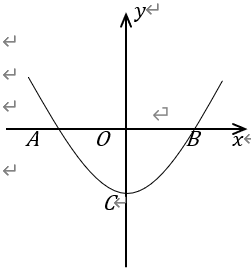
\includegraphics[width=10em]{288793-1642408835-2.jpg}
\end{figure}
\end{enumerate}

\clearpage
\end{document}
\documentclass{article}
\usepackage{pdfpages}
\usepackage[paperwidth=39.5cm,paperheight=27.2cm]{geometry}
\begin{document}
\includepdf[pages=1-6,nup=2x1]{dibajiefeishujuesaijuanzi.pdf}
\end{document}
doublepages